\documentclass[12pt,a4paper,titlepage]{article}
\usepackage[left=2.5cm,text={16cm,20cm},top=4cm]{geometry}
\usepackage[T1]{fontenc}
\usepackage[czech]{babel}
\usepackage[utf8]{inputenc}
% dalsi balicky
\usepackage{graphicx}
\usepackage{enumitem}
\usepackage{indentfirst}
\usepackage{float}
\usepackage{svg}
\usepackage{amsmath}
\usepackage{url}
\usepackage{graphics}
\usepackage{graphicx}
\usepackage{multicol}
\graphicspath{ {images/} }
\usepackage[bookmarksopen,colorlinks,plainpages=false,urlcolor=blue,
unicode,linkcolor=black]{hyperref}

\bibliographystyle{czplain}

%úvodzovky
\providecommand{\uv}[1]{\quotedblbase #1\textquotedblleft}

\begin{document}

\begin{titlepage}
\begin{center}
    {
    	\Huge\textsc{Vysoké učení technické v~Brně}}\\
    \smallskip
    {
    	\huge\textsc{Fakulta informačních technologií}}\\
    \bigskip
    \vspace{\stretch{0.382}} %pomery odpovedajúcí zlatému rezu    
    \huge{Pokročilé databázové systémy}\\
    \smallskip
    \Huge{Projekt -- map maker}\\
    \vspace{\stretch{0.618}}
\end{center}
    {\Large \today \hfill David Kozák (xkozak15)  }\\
    \smallskip
    {\Large \hfill Pavel Plaskoň (xplask00)  }\\
    \smallskip
    {\Large \hfill Jan Velecký (xvelec07)  }\\
\end{titlepage}

\newpage
\tableofcontents
\newpage

\section{Úvod}
Tato dokumentace popisuje aplikaci MapMaker, která vznikla jako projekt do předmětu Pokročilé databázové systémy v zimním semestru akademického roko 2017. Cílem tohoto programu je umožňovat uživatelům jednoduchým způsobem vytvářet mapy, které jsou interaktivní a proměnlivé v čase. Do mapy je možné vložit různé geometrické entity a poté je i upravovat. Ke každé entitě je možné přidat detaily jako jméno, popis, rozsah platnosti, geometrické detaily a sérii obrázků charakterizujících dané místo.

\section{Přeložení a spuštění aplikace}
Jedná se o JavaFX aplikaci sestavovanou jako Maven projekt. Je tedy možné ji přeložit příkazem \textit{mvn clean install}. Po překladu naleznete ve složce \textit{target} jar archiv \textit{fit-pdb17-epsilon-1.0-SNAPSHOT.jar}, ve kterém se nachází aplikace i se všemi podpůrnými knihovnami. Pro spuštění lze využít přiložený skript \textit{run.sh}. 

\section{Popis grafického uživatelského rozhraní}
Aplikace se skládá z několika oken, jmenovitě z hlavního okna, nastavení a okna \textit{about} zobrazující základní informace o aplikaci. Druhé dvě okna jsou poměrně jednoduché, důležité je hlavní okno, ve kterém se nacházejí všechny důležité komponenty. 

\begin{figure}[!htbp]
	\centering
	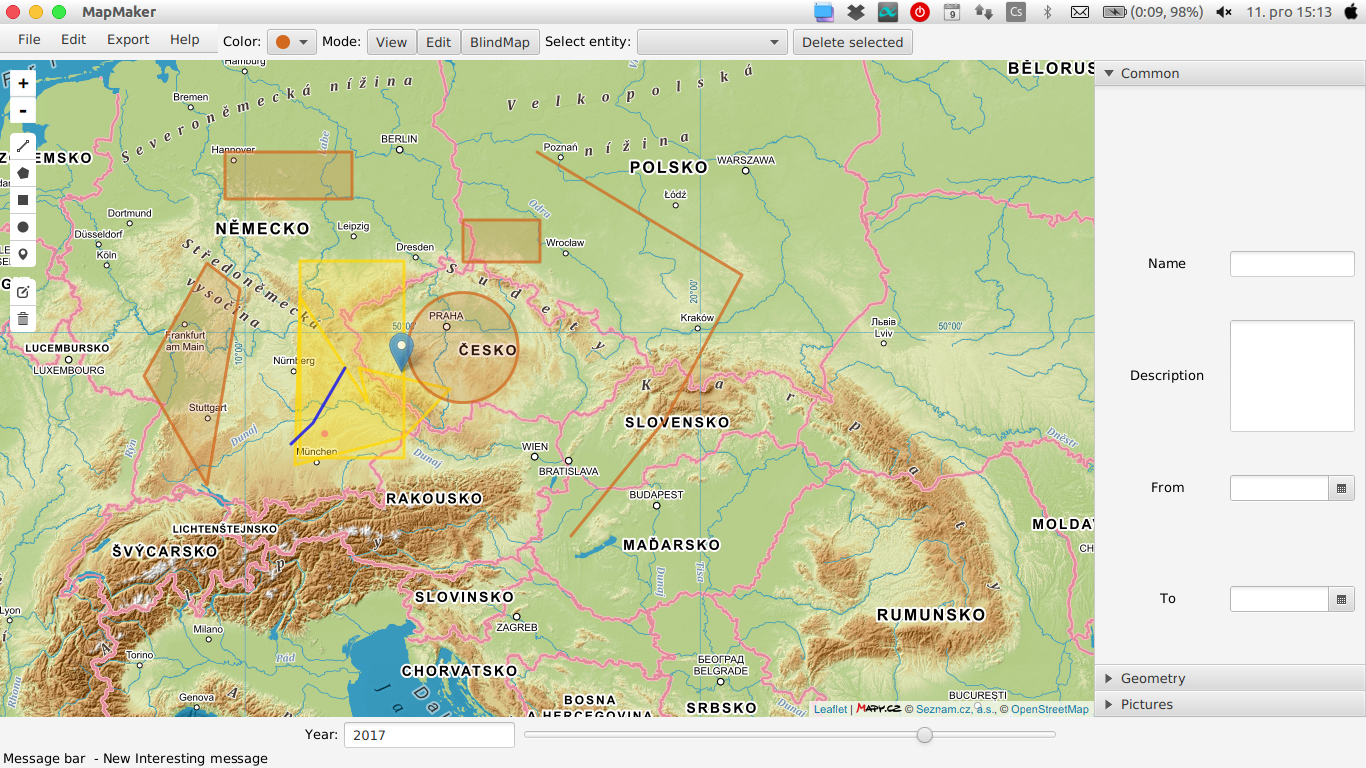
\includegraphics[scale=0.3]{full_window}
	\caption{Celé okno}
	\label{fullWindow}
\end{figure}

\subsection{Hlavní okno}
Hlavní okno sestává z několika částí. Jeho valnou většinu zabírá interaktivní mapa, přes kterou je možné přidávat nové entity do aplikace. 

Nahoře naleznete menu, přes které je možné zobrazit inicializovat databázi, zobrazit nastavení, zavřít aplikaci, smazat všechny entity, exportovat obrázek z mapy a zobrazit dialog about. 

Napravo od menu se nachází toolbar, který umožňuje změnit barvu, kterou jsou entity vykreslovány a také přepínat mezi třemi módy aplikace, view, edit a blind map. Dále je zde také možné vybrat entitu, jejíž detaily chceme editovat, a tuto entitu smazat. Stejné operace je také možné provést přes samotnou mapu.

\subsection{Pravá lišta}
Pravá lišta může mít dvě různé podoby v závislosti na módu aplikace.

V módech view a edit se zde zobrazují informace o právě zvolené entitě. Je tedy možné nově vytvořenou entitu hned editovat. 

V módu blindmap se zde zobrazuje jednoduchá hra, ve  které uživatel musí určit, který z daných tří obrázků patří ke zvolenému místu.

\begin{figure}[!htbp]
	\centering
	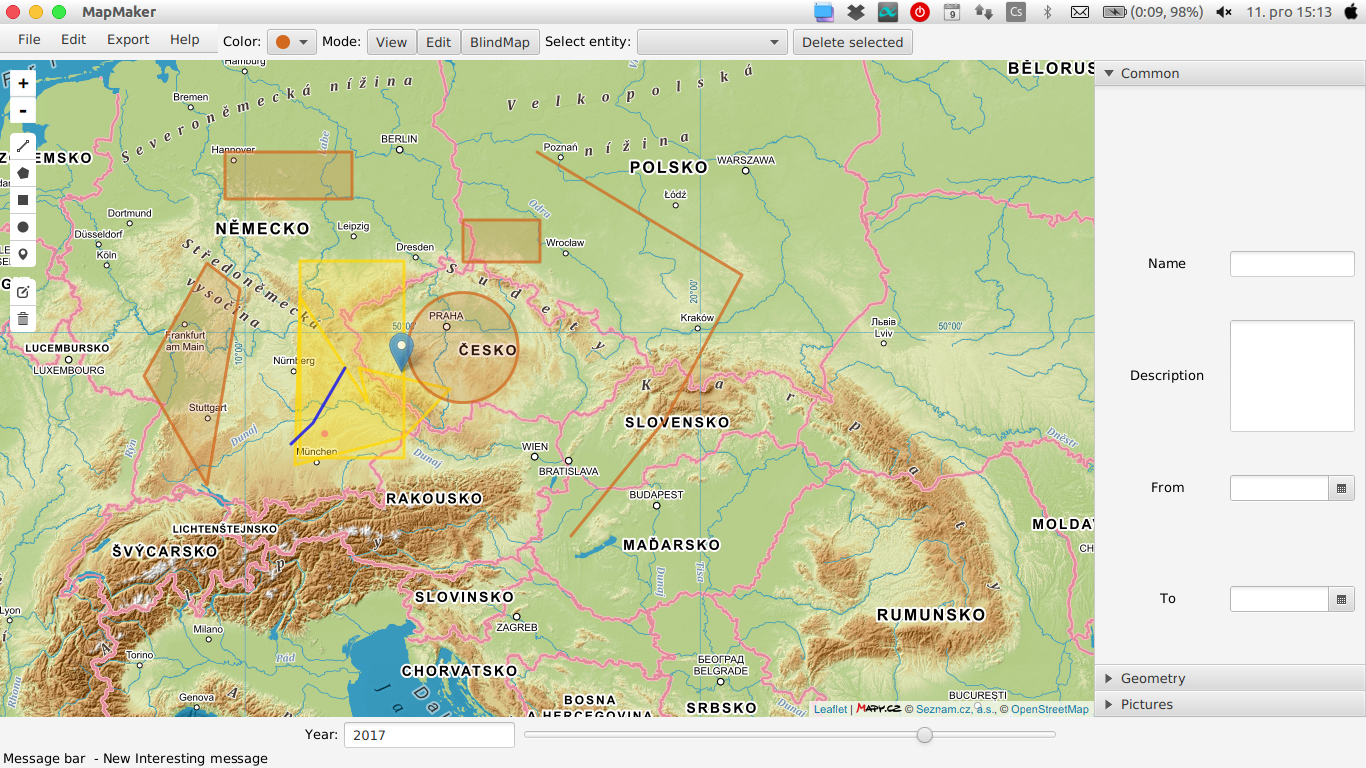
\includegraphics[scale=0.25]{full_window}
	\caption{Details pravá lišta}
	\label{rightBar}
\end{figure}

\begin{figure}[!htbp]
	\centering
	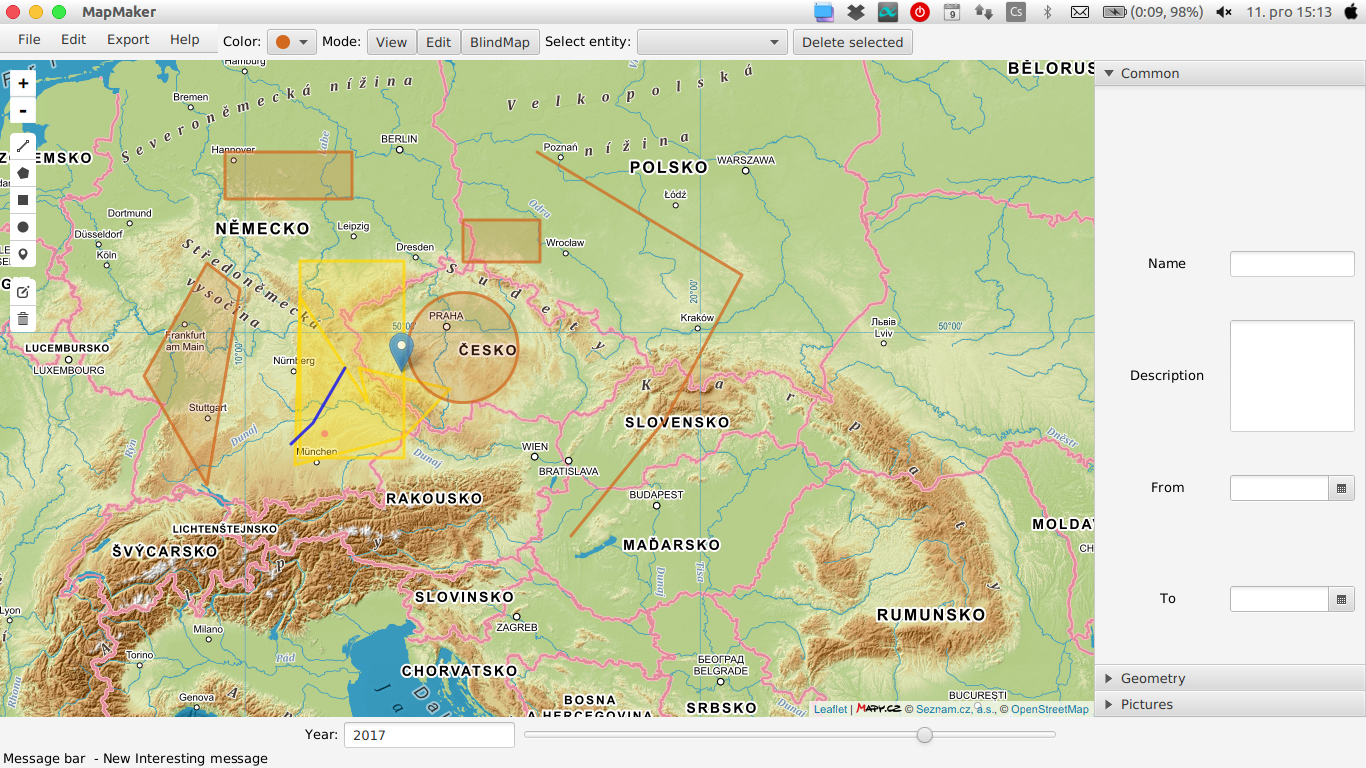
\includegraphics[scale=0.25]{full_window}
	\caption{Detail slepá mapa}
	\label{blindMap}
\end{figure}

\subsection{Nastavení}
V okně nastavení je možné změnit URI databáze a také změnit přihlašovací údaje. Při kliknutí na potvrzovací tlačítko dojde k pokusu a připojení a okno se ukončí, pouze pokud připojení proběhne úspěšně, jinak dojde k vypsání chybového hlášení a uživatel má možnost údaje upravit.

\begin{figure}[!htbp]
	\centering
	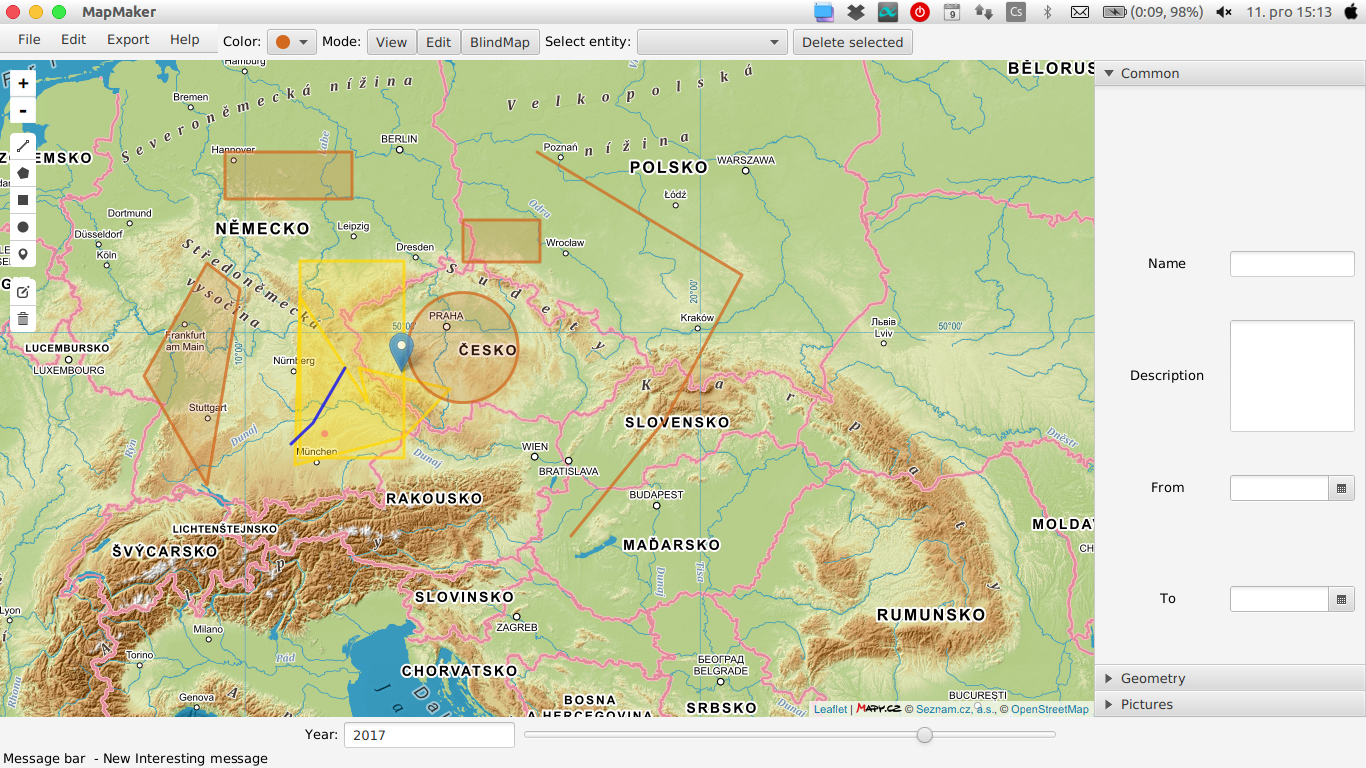
\includegraphics[scale=0.25]{full_window}
	\caption{Details nastavení}
	\label{settings}
\end{figure}

\section{Prostorové dotazy}
V této sekci se nachází popis jednotlivých dotazů a analytických funkcí, které poskytujeme uživateli jako doplňující materiál zvyšující využitelnost aplikaci.

\subsection{Složité dotazy}

\subsection{Analytické funkce}

\end{document}